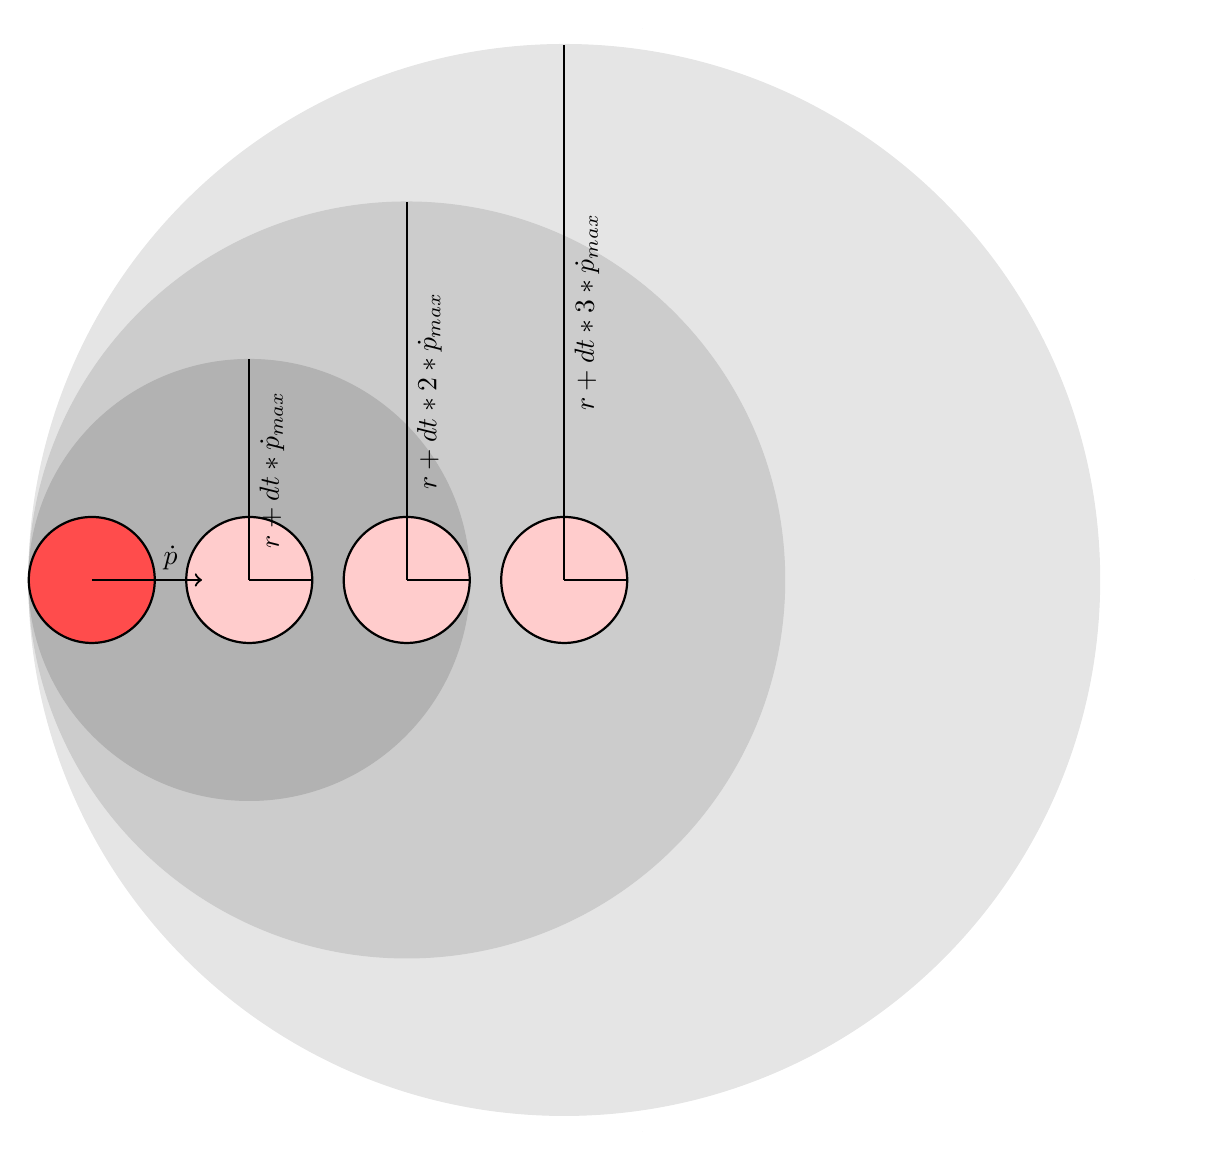
\begin{tikzpicture}
    % Define the centers and radii of the circles
    \coordinate (center1) at (0, 0);
    \coordinate (ref) at (14, 0);
    \coordinate (ref1) at (7, 7);
    \coordinate (ref2) at (7, -7);
    \filldraw[black, thick] (center1) circle(2pt);
    \filldraw[black, thick] (ref) circle(0pt);
    \filldraw[black, thick] (ref1) circle(0pt);
    \filldraw[black, thick] (ref2) circle(0pt);

    % Draw the first circle
    \draw<9->[black!10, fill=black!10] {([xshift=6cm]center1) circle (6.8cm)};
    \draw<8->[black!20, fill=black!20] {([xshift=4cm]center1) circle (4.8cm)};
    \draw<7->[black!30, fill=black!30] {([xshift=2cm]center1) circle (2.8cm)};
    \draw[black, thick, fill=red!70] (center1) circle (0.8cm);
    \draw<4->[fill=red!20, thick] {([xshift=2cm]center1) circle (0.8cm)};
    \draw<5->[fill=red!20, thick] {([xshift=4cm]center1) circle (0.8cm)};
    \draw<6->[fill=red!20, thick] {([xshift=6cm]center1) circle (0.8cm)};
    \draw<3->[->, thick]{(center1) -- ([xshift=1.4cm]center1) node[midway, above, xshift=0.3cm] () {$\dot{\boldsymbol{p}}$}};
    \draw<7->[thick]{
        ([xshift=2cm]center1) -- ([xshift=2cm, yshift=2.8cm]center1) node[midway, below, sloped] () {$r + dt * \dot{\boldsymbol{p}}_{max}$}
        ([xshift=2cm]center1) -- ([xshift=2.8cm]center1)
    };
    \draw<8->[thick]{
        ([xshift=4cm]center1) -- ([xshift=4cm, yshift=4.8cm]center1) node[midway, below, sloped] () {$r + dt * 2 * \dot{\boldsymbol{p}}_{max}$}
        ([xshift=4cm]center1) -- ([xshift=4.8cm]center1)
    };
    \draw<9->[thick]{
        ([xshift=6cm]center1) -- ([xshift=6cm, yshift=6.8cm]center1) node[midway, below, sloped] () {$r + dt * 3 * \dot{\boldsymbol{p}}_{max}$}
        ([xshift=6cm]center1) -- ([xshift=6.8cm]center1)
    };
\end{tikzpicture}
